\documentclass{beamer}
\usetheme{Copenhagen}
\usepackage{listings}
\usepackage{minted}
\usepackage{graphicx}
\usepackage{subfig}
\usepackage{macros}

\title{Implémentation du protocole CRS d'échange de clefs à base d'isogénies }
\author{Hugo Nartz, Cl\'ement Jacquot}
\date{16 F\'evrier 2022}

%Page number
\expandafter\def\expandafter\insertshorttitle\expandafter{%
  \insertshorttitle\hfill%
  \insertframenumber\,/\,\inserttotalframenumber}

%%%%%%%%%%%%%%%%%%%%%%%%%%%%%%%%%%%%%%%%%%%%%%%%%%%%%%
%% Titlepage
%%%%%%%%%%%%%%%%%%%%%%%%%%%%%%%%%%%%%%%%%%%%%%%%%%%%%%
\begin{document}
\begin{frame}
  \titlepage
\begin{figure}[h]
\centering
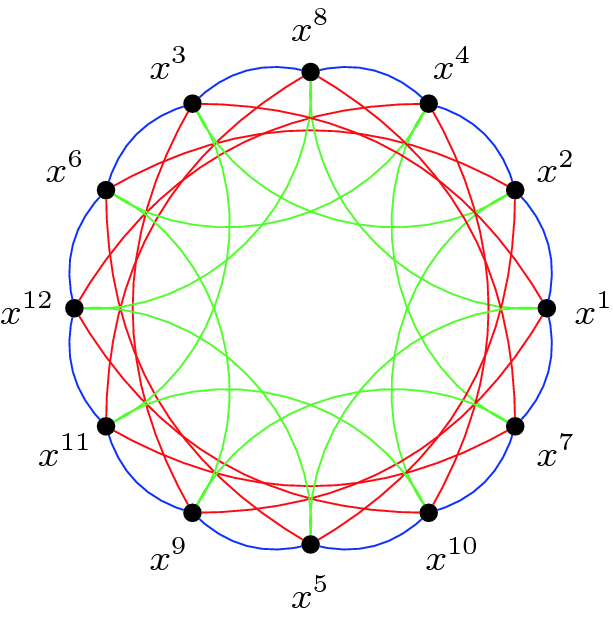
\includegraphics[scale=0.13]{../figs/isoGraph}
\end{figure}
\end{frame}

%%%%%%%%%%%%%%%%%%%%%%%%%%%%%%%%%%%%%%%%%%%%%%%%%%%%%%
%% Toc
%%%%%%%%%%%%%%%%%%%%%%%%%%%%%%%%%%%%%%%%%%%%%%%%%%%%%%
\begin{frame}{}
  \tableofcontents
\end{frame}

\section{Le protocol CRS}

%%%%%%%%%%%%%%%%%%%%%%%%%%%%%%%%%%%%%%%%%%%%%%%%%%%%%%
%% Parametres
%%%%%%%%%%%%%%%%%%%%%%%%%%%%%%%%%%%%%%%%%%%%%%%%%%%%%%
\begin{frame}{Param\`etres de base}
	Corps de base:
	\[
		\mathbb{F}_p \text{ avec } p\sim 2^{512}.
	\]
	Courbe de base avec de bonnes propri\'et\'es:
	\[
		E: Y^2 = X^3 + AX^2 + X  \text{ o\`u } A\in  \mathbb{F}_p.
	\]
	Notamment $\# E(\FFp) = 3\cdot 5\cdot 7\cdot 11 \cdot 13\cdot 17\cdots$
\end{frame}

%%%%%%%%%%%%%%%%%%%%%%%%%%%%%%%%%%%%%%%%%%%%%%%%%%%%%%
%% Isogenies
%%%%%%%%%%%%%%%%%%%%%%%%%%%%%%%%%%%%%%%%%%%%%%%%%%%%%%
\begin{frame}{Isog\'enies et Frobenius}
	\begin{itemize}
		\item  $l$: petit diviseur premier de $\#E(\FFp)$ co-premier \`a $p$.
		\item Pour  tout $P\in E(\FFp)[l]$ il existe une unique $l$-isog\'enie
	\[
		\phi: E\rightarrow E/<P>
	\]
	telle que $\ker\phi = <P>$.
\item Pour certains $l$ (\textit{Elkies primes}), le Frobenius
		\[
			\pi: (x, y)\in E[l]\mapsto (x^p, y^p)\in E[l]
		\]
	a deux valeurs propres $\lambda$ et $\mu$.
\item $E[l]$ est somme de deux sous-espaces propres de cardinaux $l$: deux isog\'enies associ\'ees.
	\end{itemize}
\end{frame}

%%%%%%%%%%%%%%%%%%%%%%%%%%%%%%%%%%%%%%%%%%%%%%%%%%%%%%
%% Graphes
%%%%%%%%%%%%%%%%%%%%%%%%%%%%%%%%%%%%%%%%%%%%%%%%%%%%%%
\begin{frame}{Graphes d'isog\'enies}
	\begin{itemize}
		\item Deux $l$-isog\'enies par courbe: deux directions ($\lambda$ et $\mu$).
		\item Isog\'enie \textit{duale} de degr\'e $l$ ($\dashrightarrow$): pour revenir en arri\`ere.
		\item Conservation des propri\'et\'es dans la composante connexe
	\end{itemize}
	 \vspace*{0.2cm}
	$\rightarrow$ Pour chaque $l$ (Elkies): un cycle dont les sommets sont des courbes elliptiques et les ar\^etes des isog\'enies.
	 \vspace*{0.2cm}
	\begin{center}
		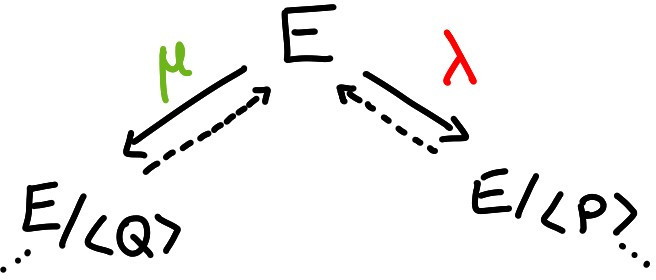
\includegraphics[scale=0.2]{../figs/Cycle}
	\end{center}
	$\rightarrow$ Les pas dans le graphe commutent par rapport aux differents $l$.
\end{frame}

%%%%%%%%%%%%%%%%%%%%%%%%%%%%%%%%%%%%%%%%%%%%%%%%%%%%%%
%% Echange de clefs
%%%%%%%%%%%%%%%%%%%%%%%%%%%%%%%%%%%%%%%%%%%%%%%%%%%%%%
\begin{frame}{L'\'echange de clefs}
	\begin{itemize}
		\item Clef priv\'ee $s$: nombre de pas (al\'eatoire) pour chaque $l$.
		\item Clef publique: marche suivant les pas de la clef secr\`ete $s\curvearrowright E$.
	\end{itemize}
	 %\vspace*{0.2cm}
\begin{center}
	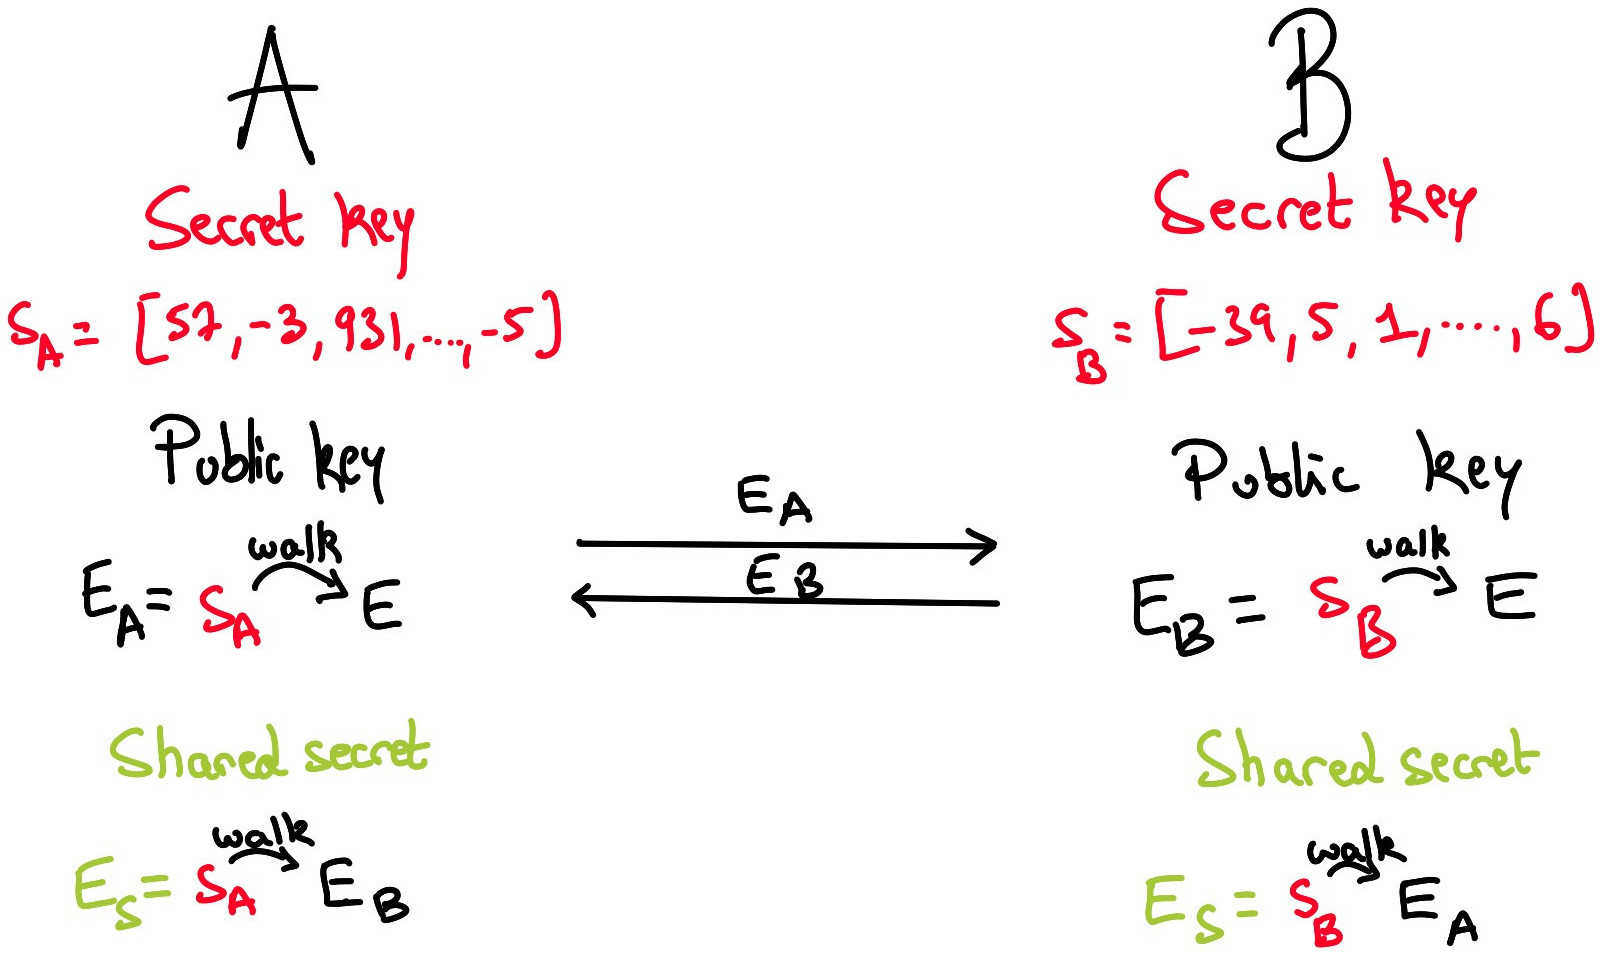
\includegraphics[scale=0.2]{../figs/DH}
\end{center}
\end{frame}

\subsection{Conclusion}
\begin{frame}
\end{frame}

\end{document}
